\mbox{$\displaystyle $\,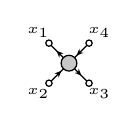
\begin{tikzpicture}[x=0.500cm, y=0.500cm, line width=0.450pt, baseline={([yshift=-0.6ex]0,0)}]
  \draw (0.000,0.000) -- (-0.509,0.509);
  \fill (-0.316,0.316) -- (-0.246,0.140) -- (-0.233,0.233) -- (-0.140,0.246) -- cycle;
  \draw (0.000,0.000) -- (0.509,-0.509);
  \fill (0.316,-0.316) -- (0.246,-0.140) -- (0.233,-0.233) -- (0.140,-0.246) -- cycle;
  \draw (-0.509,-0.509) -- (0.000,0.000);
  \fill (-0.193,-0.193) -- (-0.369,-0.264) -- (-0.276,-0.276) -- (-0.264,-0.369) -- cycle;
  \draw (0.509,0.509) -- (0.000,0.000);
  \fill (0.193,0.193) -- (0.369,0.264) -- (0.276,0.276) -- (0.264,0.369) -- cycle;
  \draw[fill=black!22] (0.000,0.000) circle (0.200);
  \draw[fill=white] (-0.509,0.509) circle (0.080);
  \draw[fill=white] (-0.509,-0.509) circle (0.080);
  \draw[fill=white] (0.509,-0.509) circle (0.080);
  \draw[fill=white] (0.509,0.509) circle (0.080);
  \node[font=\tiny, inner sep=0pt, anchor=315] at (-0.629,0.629) {$x_{1}$};
  \node[font=\tiny, inner sep=0pt, anchor=45] at (-0.629,-0.629) {$x_{2}$};
  \node[font=\tiny, inner sep=0pt, anchor=135] at (0.629,-0.629) {$x_{3}$};
  \node[font=\tiny, inner sep=0pt, anchor=225] at (0.629,0.629) {$x_{4}$};
\end{tikzpicture}}
